\documentclass{acm_proc_article-sp}

\usepackage{hyperref}

\begin{document}

\title{Thinking model and machine understanding of English primitive texts and it's application in Infrastructure as Service domain.}

\numberofauthors{3}
\author{
% 1st. author
\alignauthor Alexander Toschev\\
       \affaddr{Kazan State University}\\
       \affaddr{Universitetskaya 17,}\\
       \affaddr{420008 Kazan, Russia}
       \email{alexander.toschev@gmail.com}
% 2nd. author
\alignauthor Max Talanov\\
       \affaddr{Kazan State University}\\
       \affaddr{Universitetskaya 17,}\\
       \affaddr{420008 Kazan, Russia}
       \email{max.talanov@gmail.com}
% 3rd. author
\alignauthor Andrey Krekhov\\
       \affaddr{Fujitsu GDC Russia, Kazan}\\
       \affaddr{Sibirskii trakt 34,}\\
       \affaddr{420029 Kazan, Russia}
       \email{andrey.krekhov@ts.fujitsu.com}
}

\date{22 February 2013}

\maketitle

\begin{abstract}

Construction of machine understanding is definitely the challenge. There are several technologies used widely.
Currently mainstream applications uses machine operatable knowledge bases, for example \href{http://www.wolframalpha.com}{Wolfram Alpha} to support simple dialog and operate devices.
Newer the less those approaches do not create machine understanding of even primitive incidents.
We tried new approach based on assumption that human understanding is tightly coupled with human thinking itself.
We used thinking model described in Marvin Minsky book \href{http://en.wikipedia.org/wiki/The_Emotion_Machine}{"The emotion machine"}.

\keywords{AI, machine understanding, it outsourcing}

\end{abstract}

\section{The emotion machine thinking model}
\subsection{6 thinking levels}

\href{http://web.media.mit.edu/~minsky/E5/eb5.html}{Marvin Minsky} introduces the thinking as layered model that contains 6 layers:

\includegraphics{model_6.png}

\begin{itemize}
 \item \emph{Instinctive Reactions}:  Joan hears a sound and turns her head. All animals are born equipped with ‘instincts’ that help them to survive.
 \item \emph{Learned Reactions}: She sees a quickly oncoming car. Joan had to learn that conditions like this demand specific ways to react.
 \item \emph{Deliberative Thinking}: To decide what to say at the meeting, she considers several alternatives, and tries to decide which would be best.
 \item \emph{Reflective Thinking}: Joan reflects upon what she has done. She reacts, not just to things in things in the world, but also to recent events in her brain.
 \item \emph{Self-Reflective Thinking}: Being “uneasy about arriving late” requires her to keep track of the plans that she’s made for herself.
 \item \emph{Self-Conscious Thinking}: When asking what her friends think of her, she also asks how her actions concord with ideals she has set for herself.
\end{itemize}

Each upper layer controls lower layers, and is based on constructs and uses signals of lower layers as input.

\subsection{Selector, Critic, Way to think triple}

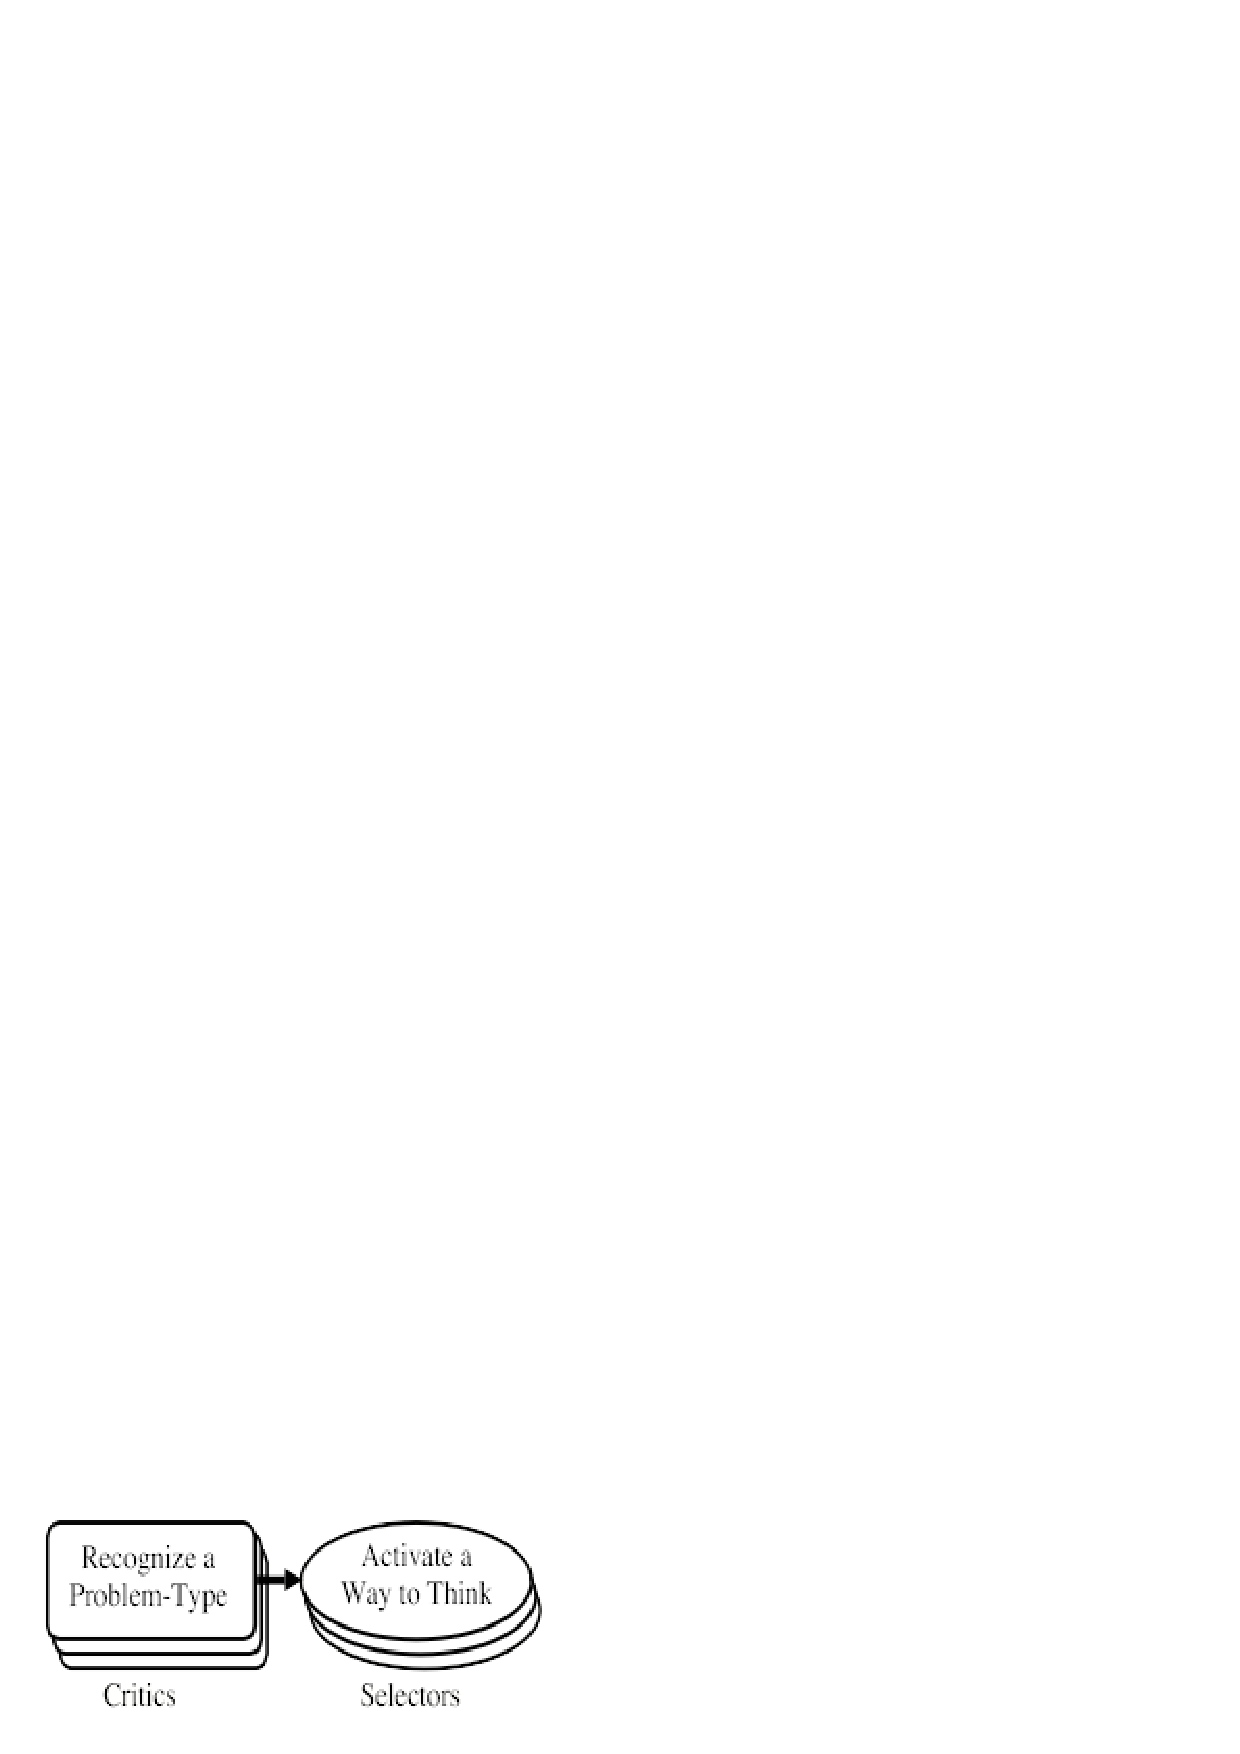
\includegraphics{critic_selector_model.png}


Marvin Minsky defines Critics - Selector behaviour as following:\\
On the left are resources that we shall call Critics, each of which can recognize a certain species of "Problem-Type". When a Critic sees enough evidence that you now are facing its type of problem, then that Critic will try to activate a "Way to Think" that may be useful in this situation.

\includegraphics{critic_selector.png}

Critic -> Selector -> Way to think are main components that implements all the machine understanding process. Critics could be understood as probabilistic predicates that does analysis of current context in memory. Selector retrieves resources from memory. Way to think is main worker that updates current context in memory.

\section{Implementation of thinking model}
\subsection{Thinking levels control}
\subsection{Memory: short term, long term}


\section{IS domain application of the thinking model}
\subsection{Critics and ways to think for incident processing}

\section{Practical results}
\subsection{Direct instruction processing}
\subsection{Problem description processing}


\subsection{References}

\end{document}